% Fragmento LaTeX para inserir no artigo IEEE/Overleaf.
% Pacotes no preambulo: \usepackage{graphicx} e \usepackage{booktabs}
% Copie outputs/ para o Overleaf preservando a estrutura de pastas.

\begin{table}[!t]
\caption{Canais de exposicao a conteudos sobre jogos de azar}
\label{tab:canais-questionario}
\centering\footnotesize
\begin{tabular}{lr}
\toprule
Canal & Mencoes \\
\midrule
Instagram & 78 \\
YouTube & 47 \\
Influenciadores & 42 \\
Amigos/conhecidos & 33 \\
TikTok & 32 \\
Sites esportivos & 27 \\
Facebook & 16 \\
Outro & 13 \\
X/Twitter & 12 \\
Nao me lembro & 2 \\
\bottomrule
\end{tabular}
\par\small Nota: questao de multipla escolha; uma pessoa podia indicar mais de um canal. "Nao me lembro" nao integra os nove canais do grafo.
\end{table}

\begin{figure}[!t]
\centering
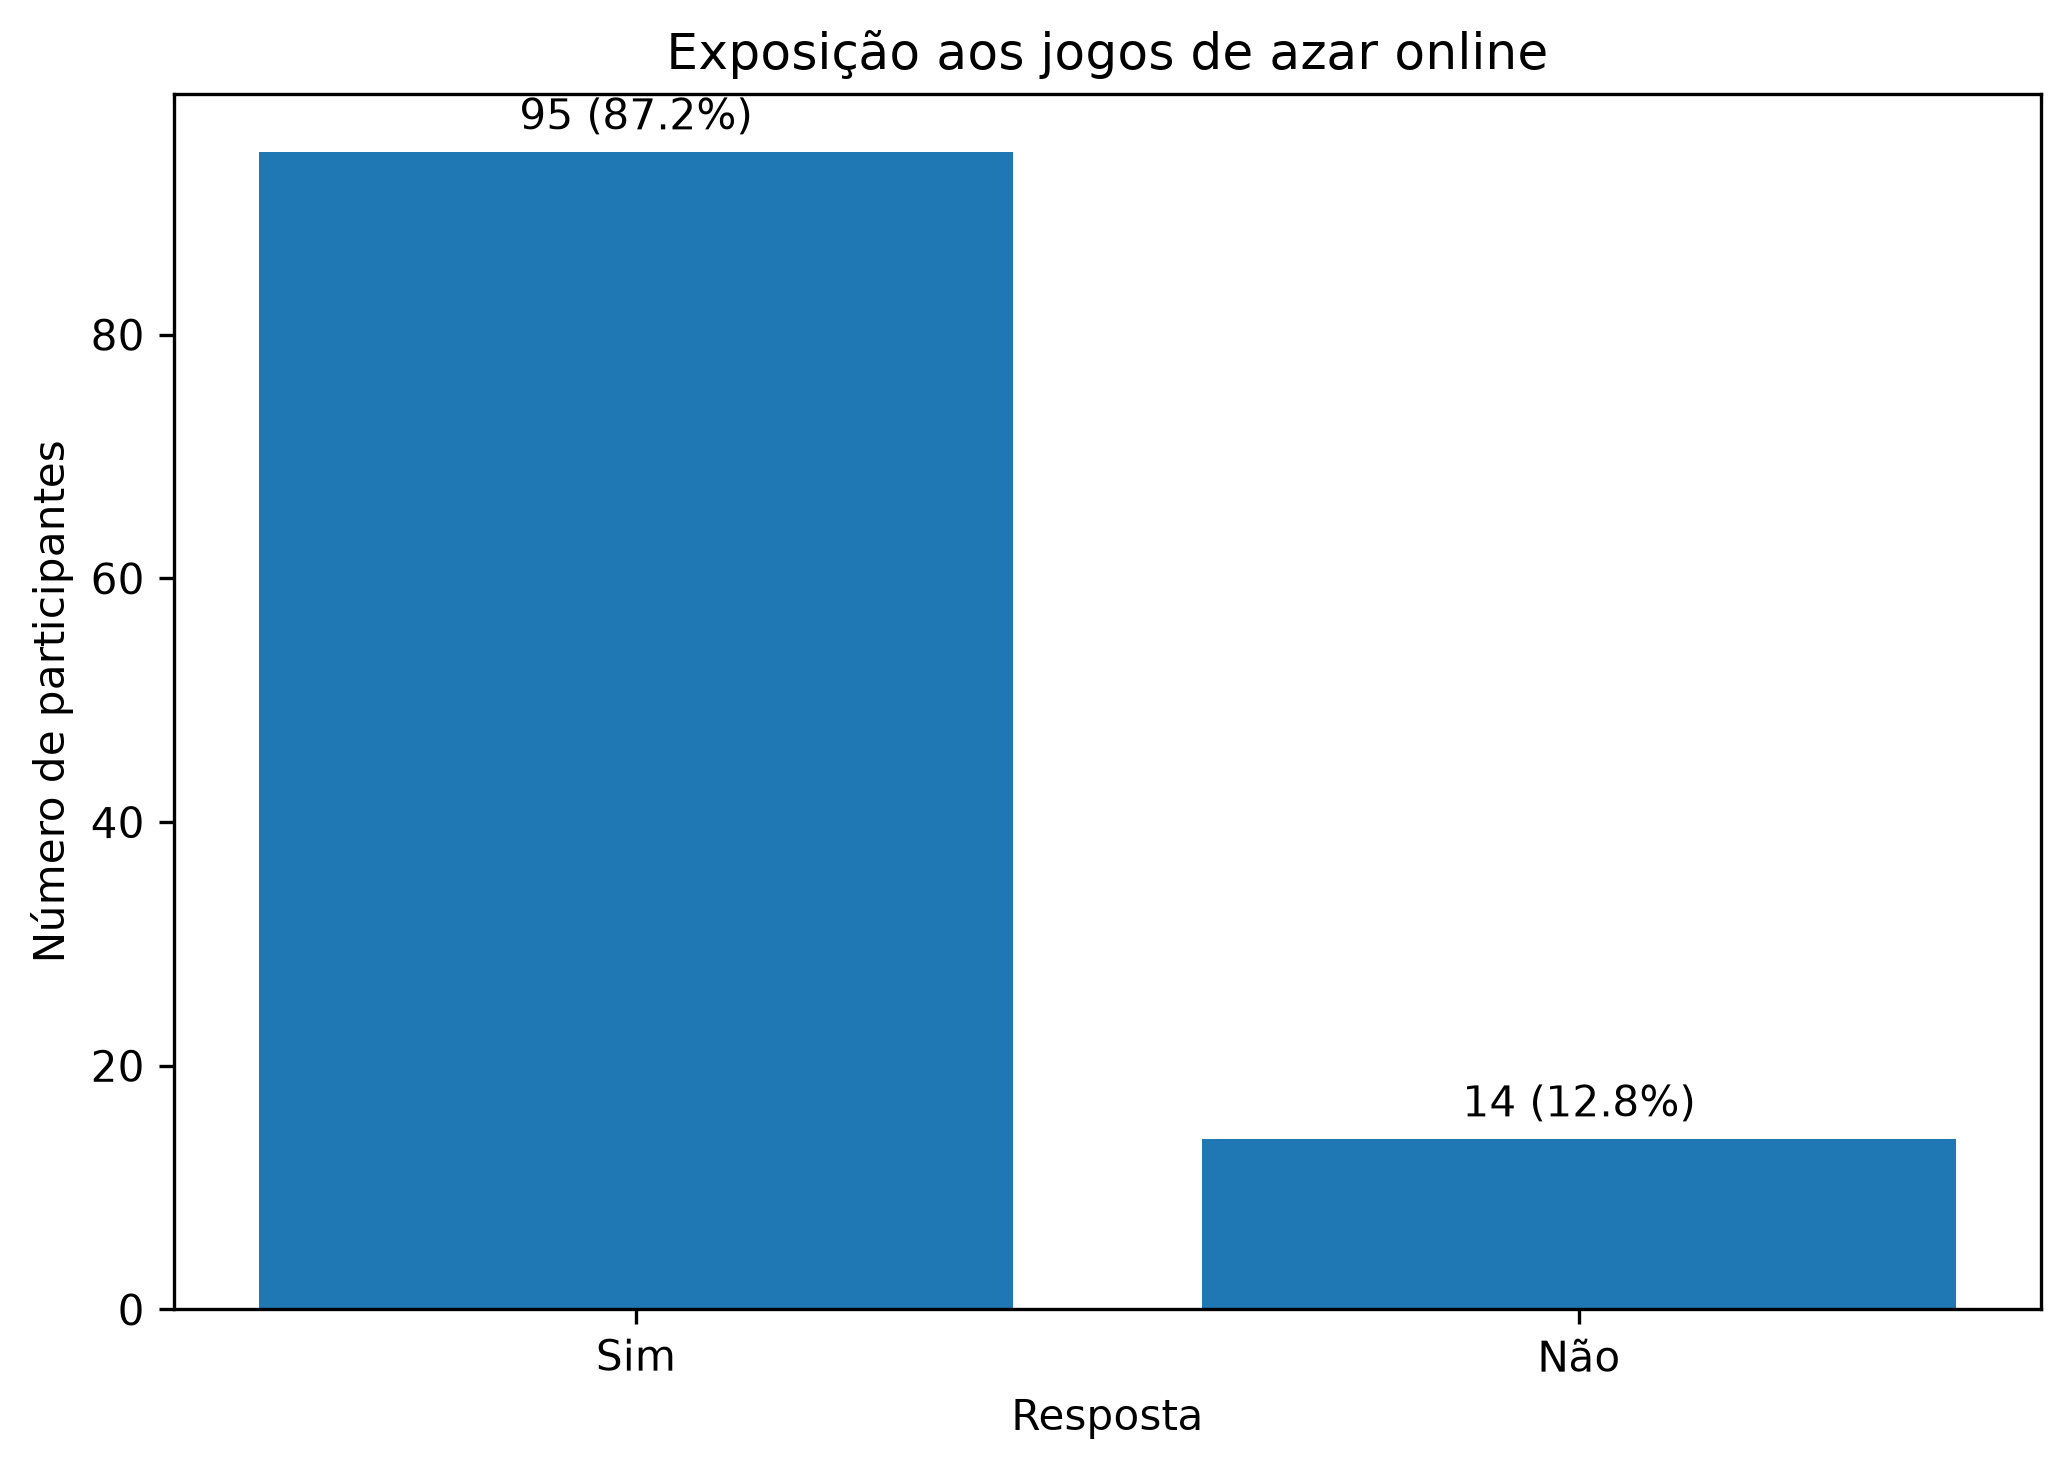
\includegraphics[width=\columnwidth]{outputs/questionario/exposicao_jogos_azar.png}
\caption{Exposicao autorrelatada a conteudos sobre jogos de azar entre os participantes do questionario.}
\label{fig:exposicao-questionario}
\end{figure}

\begin{figure}[!t]
\centering
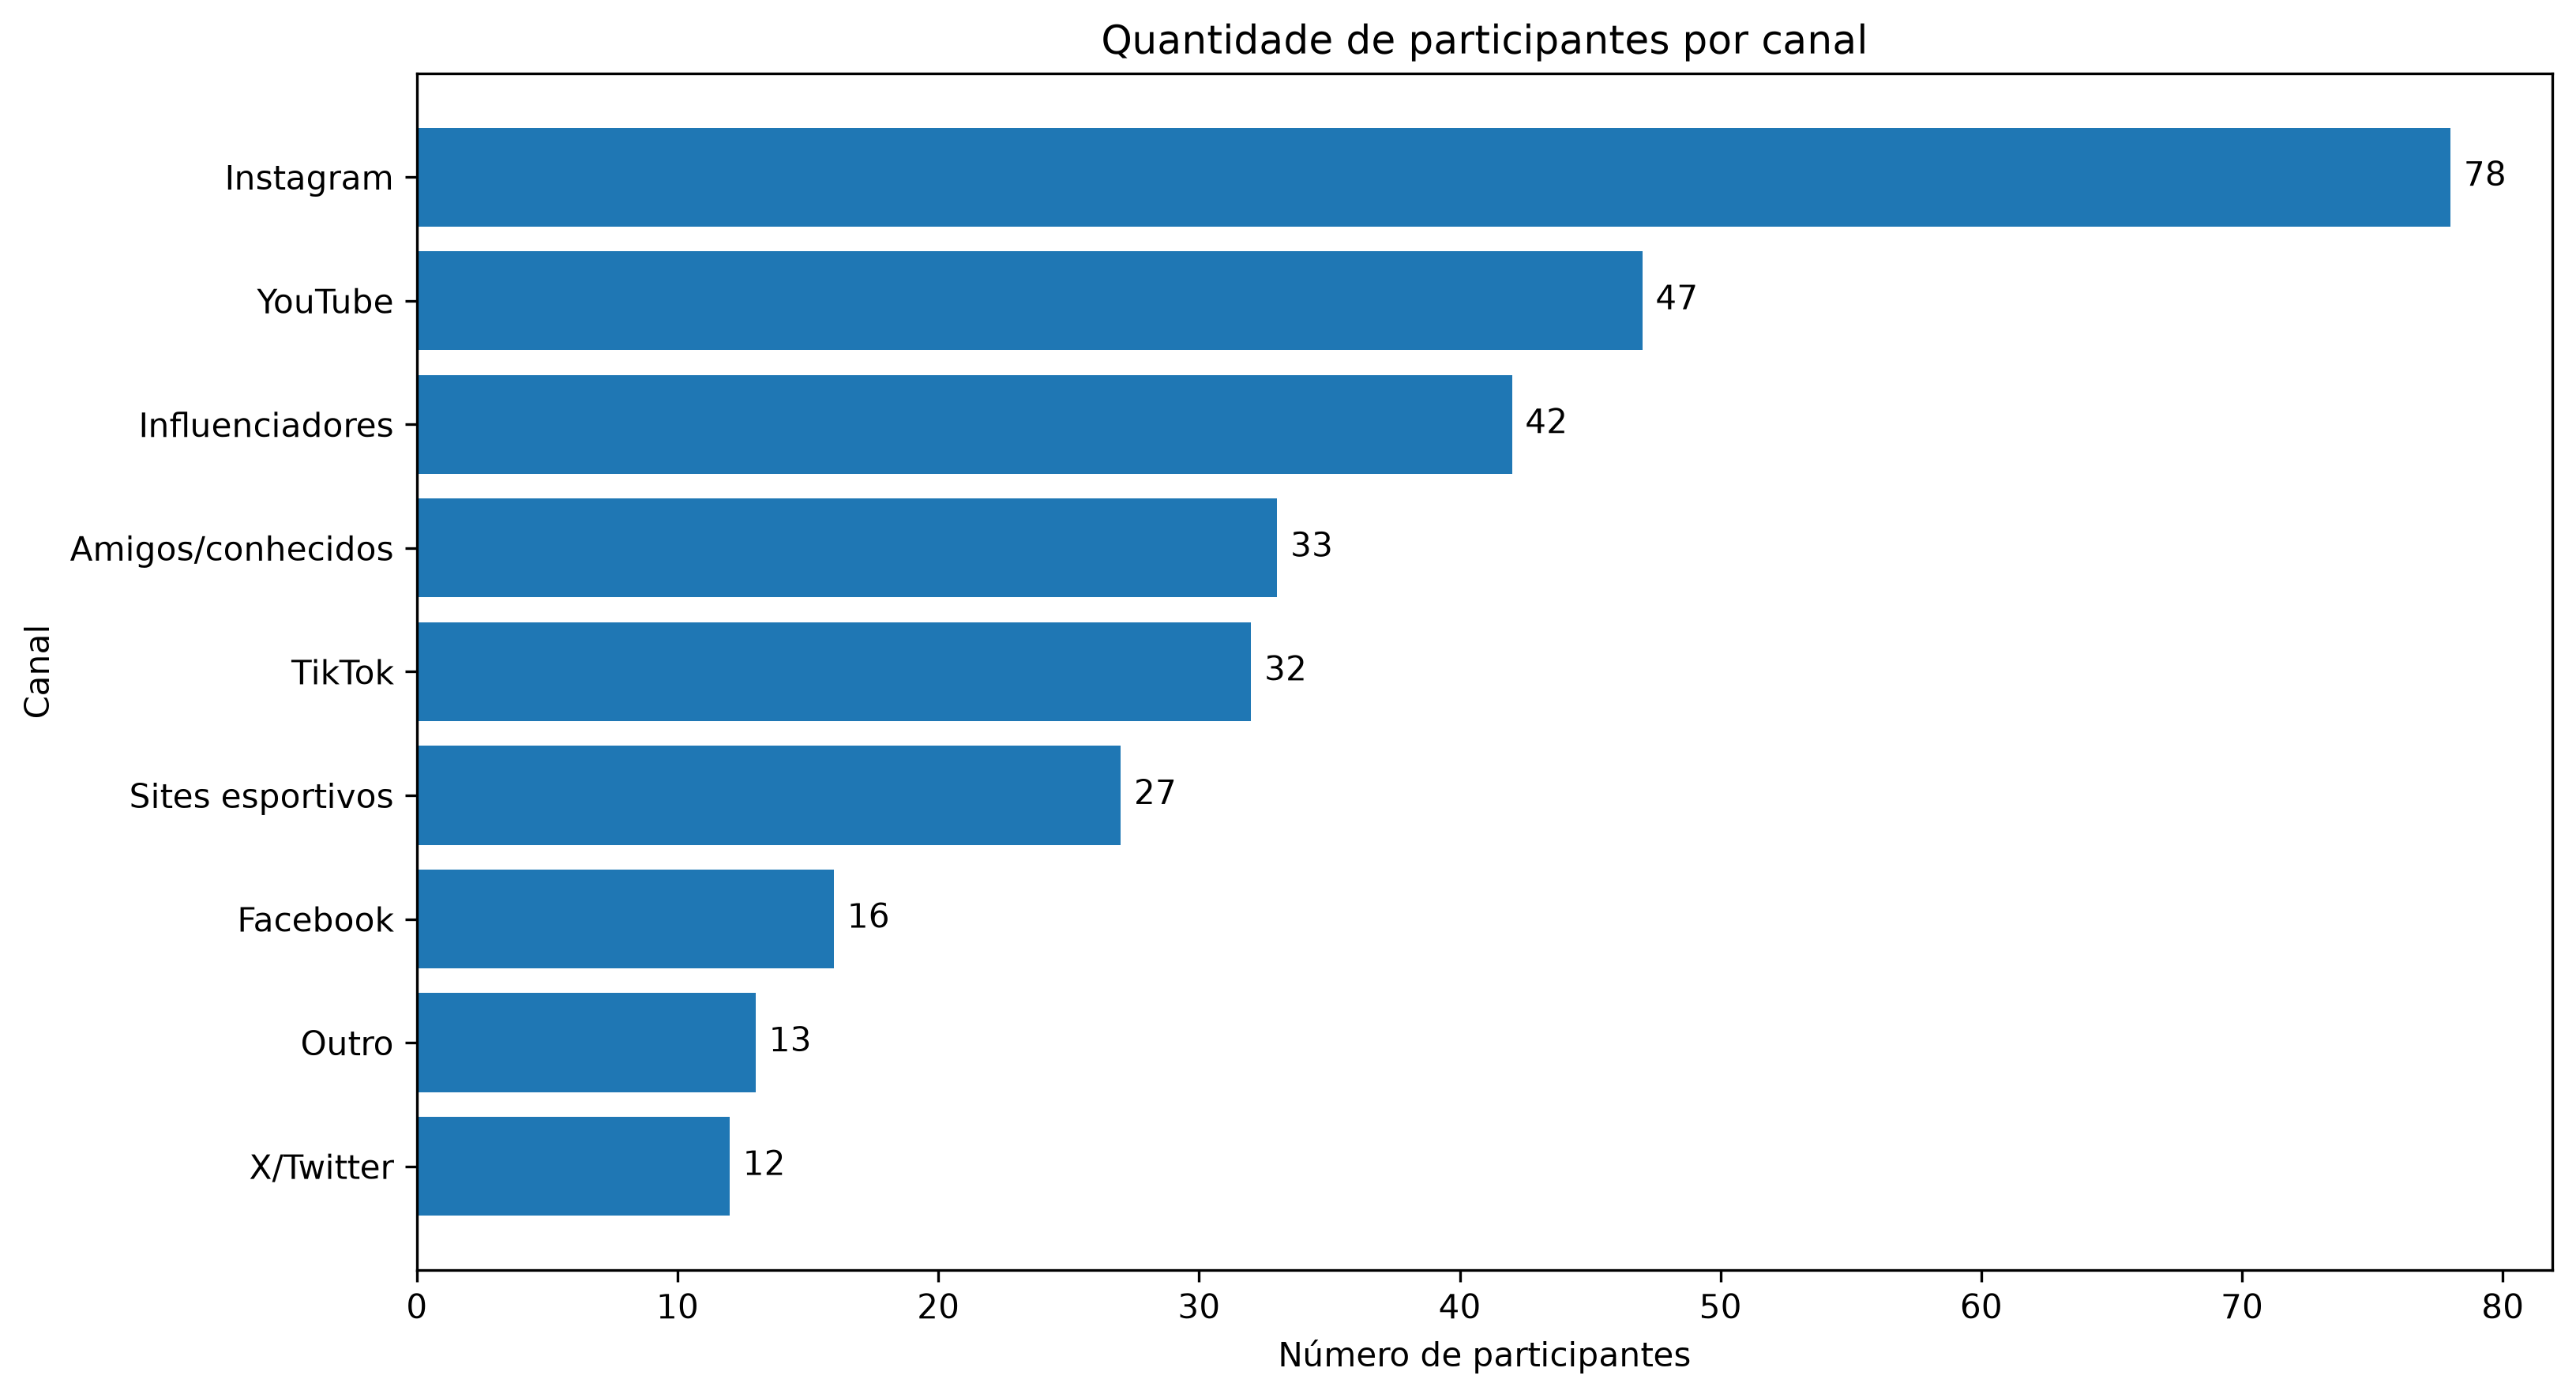
\includegraphics[width=\columnwidth]{outputs/questionario/ranking_canais.png}
\caption{Frequencia de mencoes aos canais de contato com conteudos sobre jogos de azar.}
\label{fig:ranking-canais}
\end{figure}

\begin{figure*}[!t]
\centering
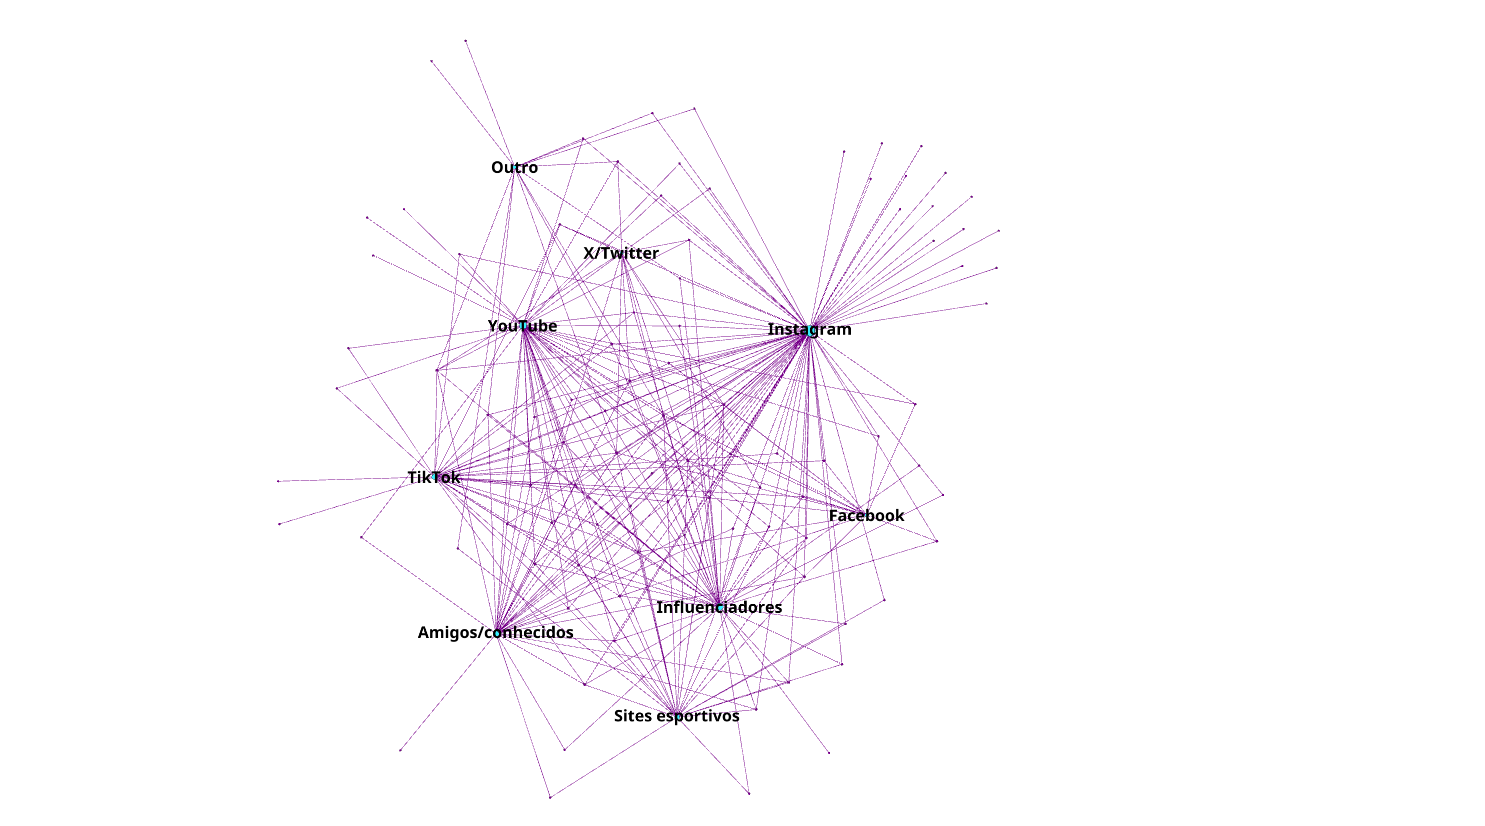
\includegraphics[width=0.88\textwidth]{outputs/questionario/grafo_gephi.png}
\caption{Rede bipartida de participantes e canais de exposicao identificados no questionario.}
\label{fig:grafo-questionario}
\end{figure*}

\begin{table}[!t]
\caption{Metricas da rede bipartida do questionario}
\label{tab:metricas-questionario}
\centering\footnotesize
\begin{tabular}{lr}
\toprule
Metrica & Valor \\
\midrule
Participantes & 109 \\
Canais & 9 \\
Vertices & 118 \\
Arestas & 300 \\
Componentes conexas & 16 \\
Maior componente & 103 vertices \\
Participantes isolados & 15 \\
\bottomrule
\end{tabular}
\end{table}

\begin{table}[!t]
\caption{Sintese da rede de recomendacoes documentadas no Telegram}
\label{tab:metricas-telegram}
\centering\footnotesize
\begin{tabular}{lr}
\toprule
Metrica & Valor \\
\midrule
Comunidades/canais representados & 14 \\
Relacoes de recomendacao & 12 \\
Componentes fracamente conexas & 2 \\
Maior componente & 10 vertices \\
Menor componente & 4 vertices \\
Densidade dirigida & 6,59\% \\
Grau medio de entrada & 0,86 \\
Grau medio de saida & 0,86 \\
\bottomrule
\end{tabular}
\par\small Nota: representa somente as relacoes identificadas nos exemplos documentados no relatorio consultado; nao corresponde ao universo completo do Telegram. As relacoes nao demonstram migracao de usuarios nem efeito causal de influencia.
\end{table}

\begin{table}[!t]
\caption{Distribuicao das relacoes documentadas por componente}
\label{tab:componentes-telegram}
\centering\footnotesize
\begin{tabular}{lrr}
\toprule
Componente & Vertices & Relacoes \\
\midrule
FORTUNE TIGIR B2XBET & 10 & 9 \\
Brasil Apostas Esportivas Palpites & 4 & 3 \\
\bottomrule
\end{tabular}
\end{table}

% Figura Telegram pendente: inserir quando existir
% outputs/telegram/rede_recomendacoes_telegram.png

\begin{table}[!t]
\caption{Classificacao de risco pelo PGSI entre apostadores recentes}
\label{tab:pgsi-lenad}
\centering\footnotesize
\begin{tabular}{lr}
\toprule
Classificacao & Percentual \\
\midrule
Sem risco & 61,4\% \\
Baixo risco & 19,4\% \\
Risco moderado & 14,8\% \\
Jogo problematico & 4,4\% \\
\bottomrule
\end{tabular}
\par\small Nota: entre os 684 respondentes que relataram apostas nos ultimos 12 meses. O PGSI e instrumento de rastreio/classificacao de risco, nao diagnostico clinico.
\end{table}

\begin{figure}[!t]
\centering
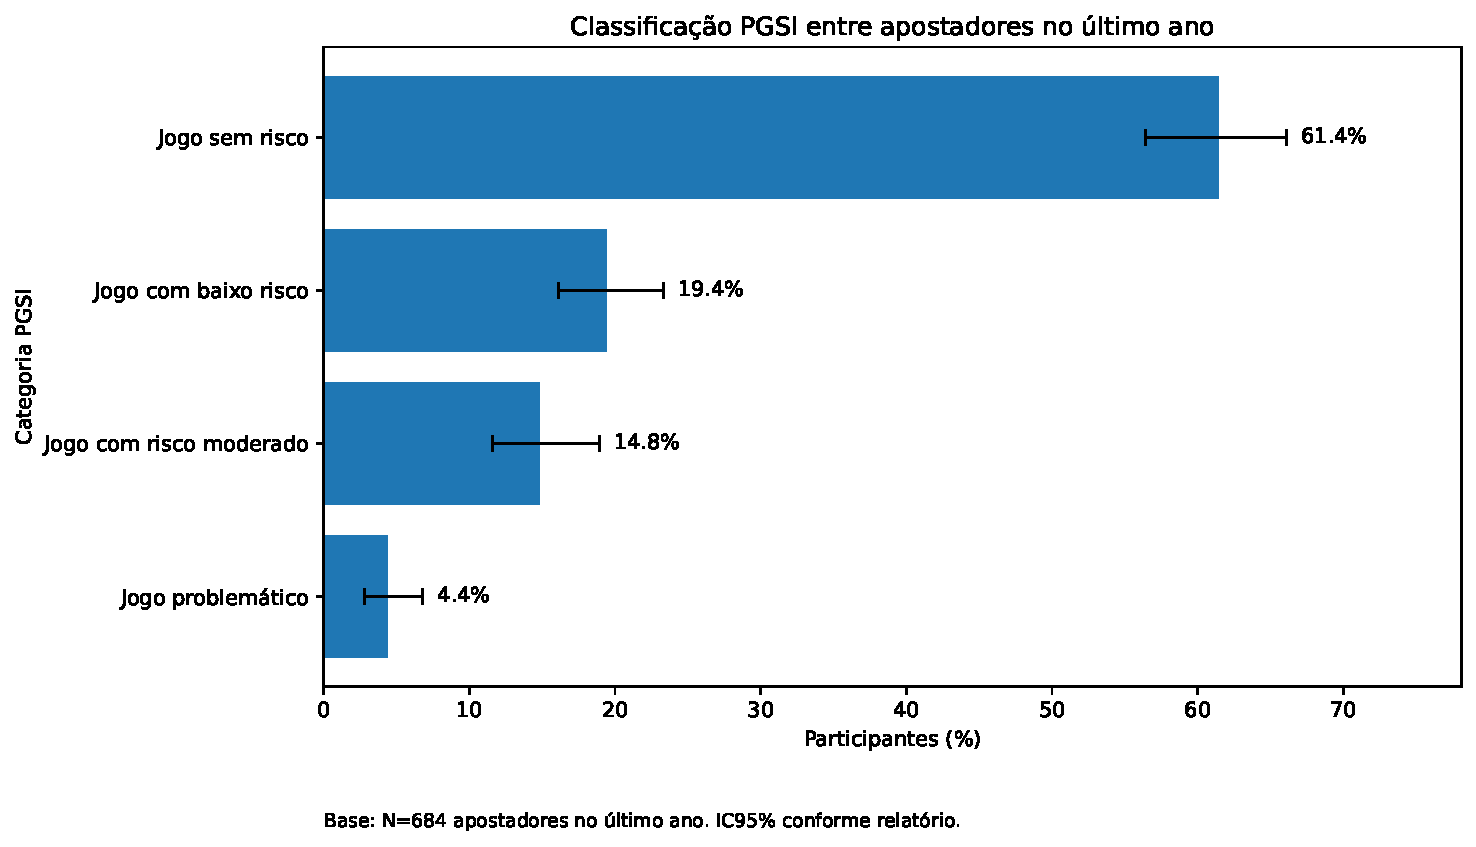
\includegraphics[width=\columnwidth]{outputs/lenad/lenad_01_classificacao_pgsi.pdf}
\caption{Distribuicao das categorias de risco segundo o PGSI no LENAD III.}
\label{fig:pgsi-lenad}
\end{figure}

\begin{figure}[!t]
\centering
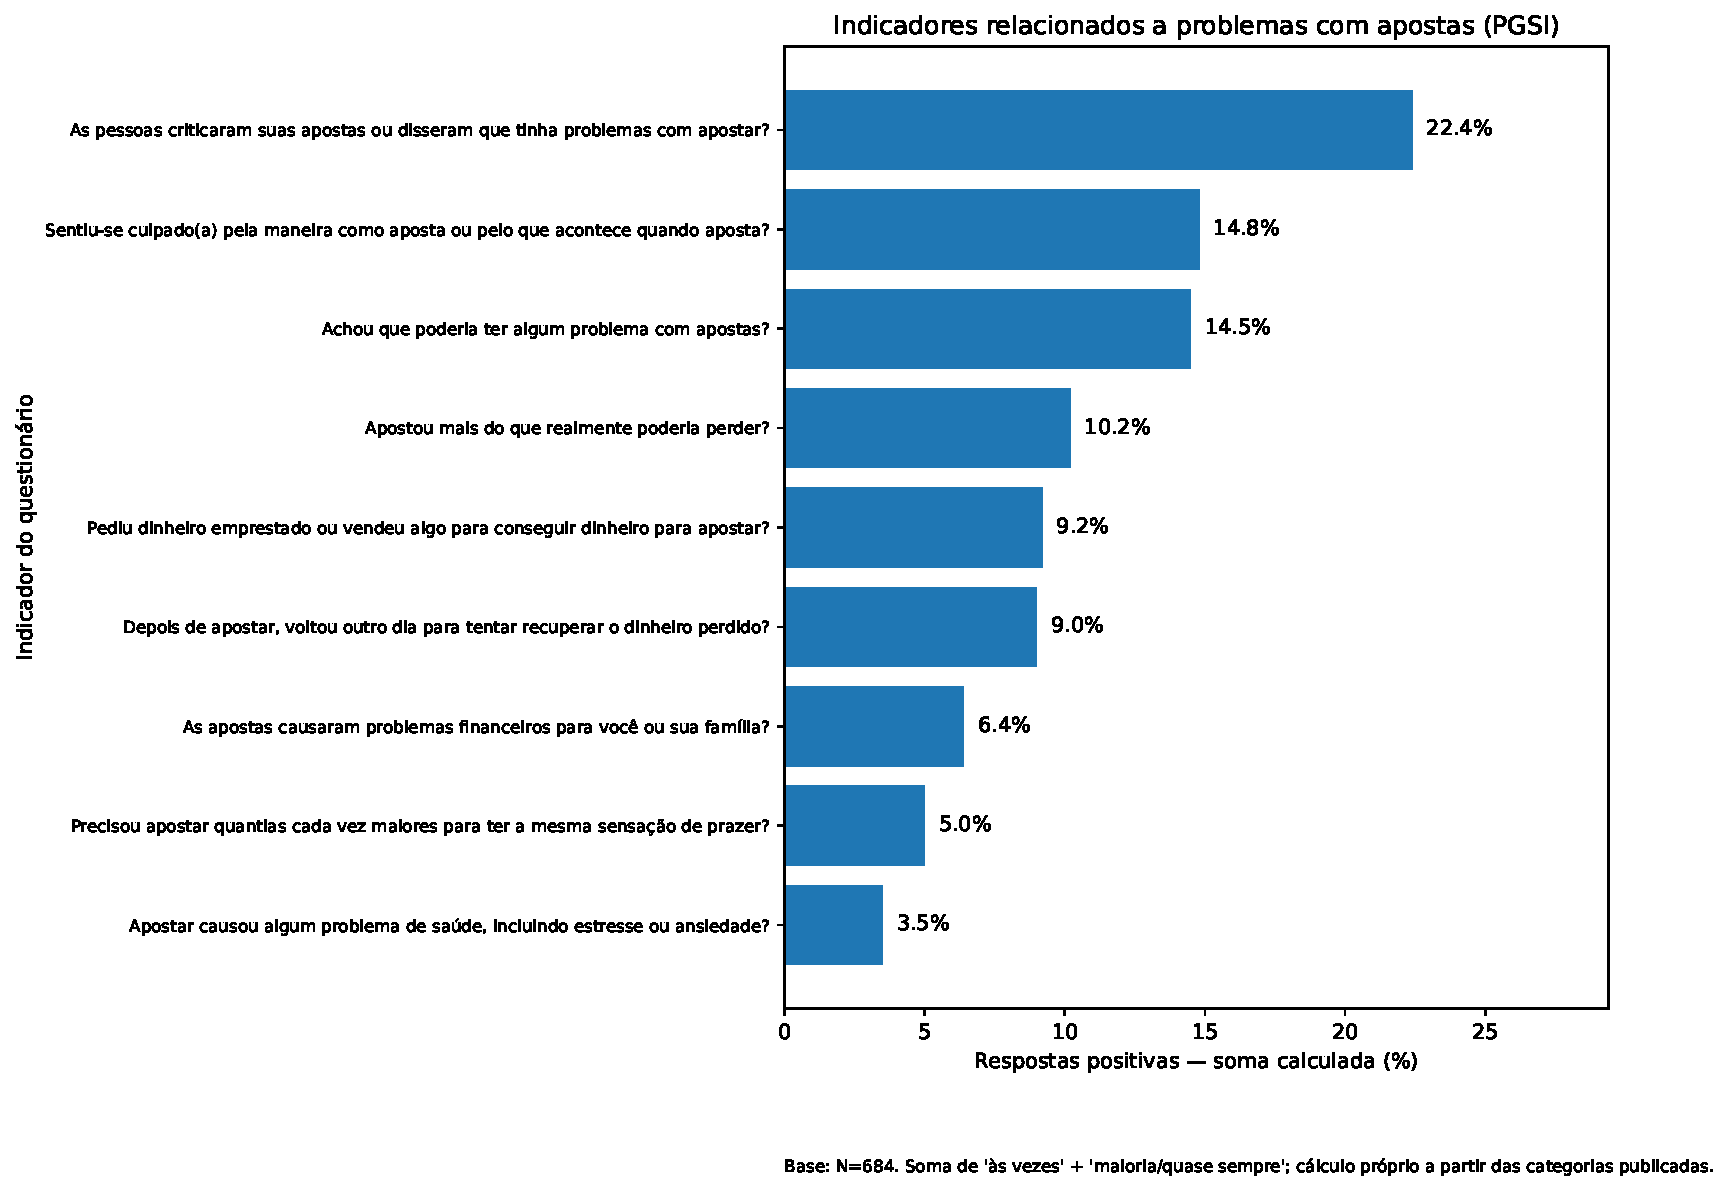
\includegraphics[width=\columnwidth]{outputs/lenad/lenad_02_indicadores_pgsi.pdf}
\caption{Indicadores autorrelatados relacionados ao comportamento de aposta no LENAD III.}
\label{fig:indicadores-lenad}
\end{figure}

\begin{table}[!t]
\caption{Classificacao de risco segundo a modalidade de aposta}
\label{tab:modalidade-lenad}
\centering\footnotesize
\begin{tabular}{lr}
\toprule
Modalidade & Com um ou mais criterios de risco \\
\midrule
Plataformas digitais (Bets) & 66,8\% \\
Outras modalidades, exceto Bets & 26,8\% \\
\bottomrule
\end{tabular}
\par\small Nota: diferenca reportada como estatisticamente significativa no material do LENAD III ($p<0{,}05$). A comparacao nao demonstra causalidade.
\end{table}

\begin{figure}[!t]
\centering
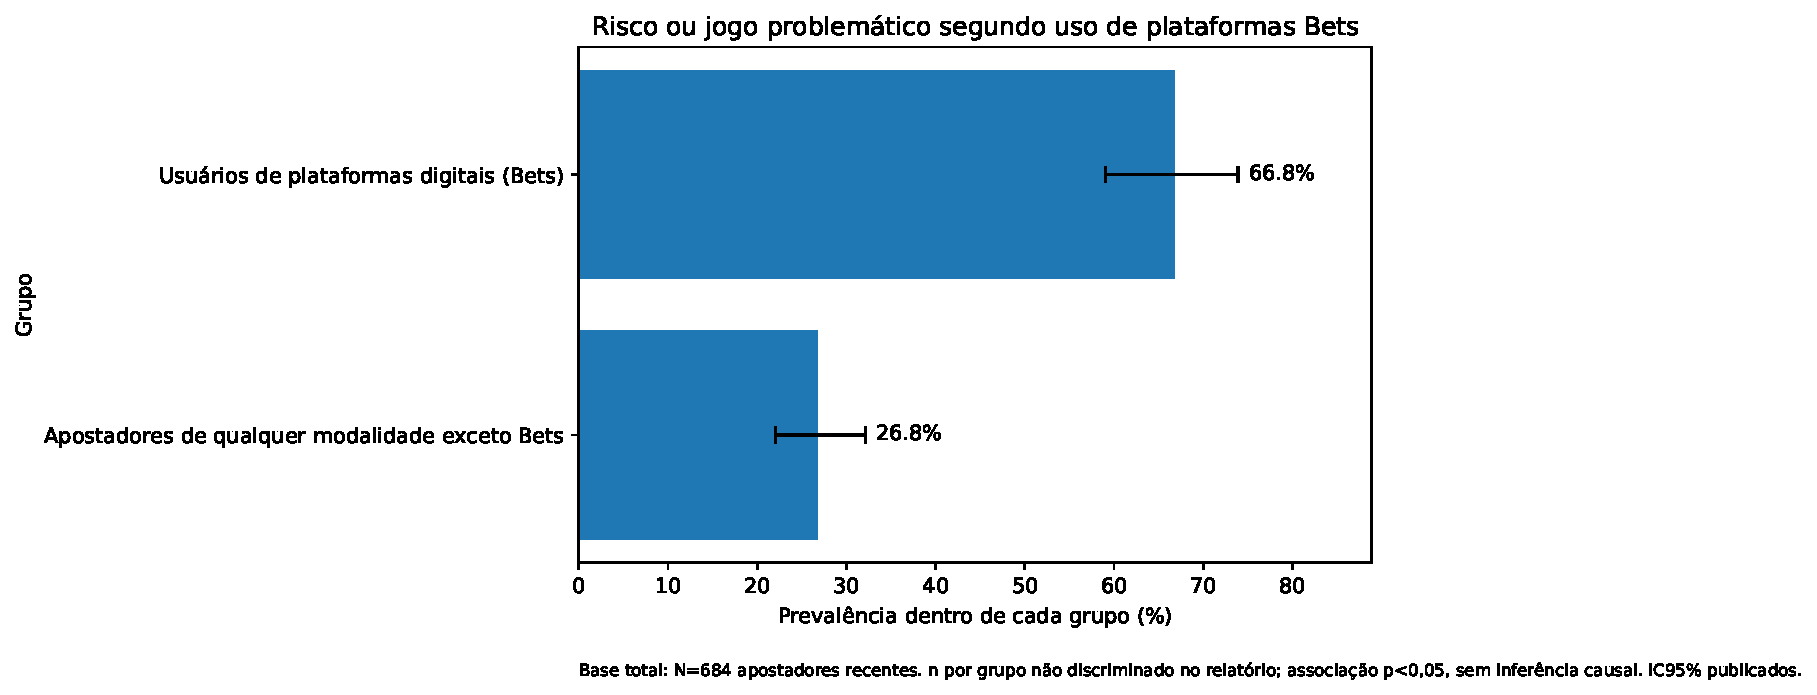
\includegraphics[width=\columnwidth]{outputs/lenad/lenad_04_risco_uso_bets.pdf}
\caption{Indicadores de risco segundo o uso de plataformas digitais de apostas (Bets).}
\label{fig:risco-bets-lenad}
\end{figure}
